\section{Unitary       transformations       and      the       rotating
  frame\label{sec:unitary}}
The Hermitian conjugate of an operator is defined as

 \begin{equation}\label{uniHermetian}
   U^{\dagger} = (U^{*})^{T},
 \end{equation}

 \noindent and the operator can be classified under two types

 \begin{itemize}
 \item $ U^{\dagger}\equiv U $ a Hermitian operator;
 \item $ U^{\dagger}\equiv U^{-1} $ is a unitary operator.
 \end{itemize}

 The most important equation for unitary operators is

 \begin{equation}\label{uniDef}
   U^{\dagger}U=\mathbb{I},
 \end{equation}

 \noindent    examples    of    which   are    Pauli    spin    matrices
 $ \sigma_x, \sigma_y, \sigma_z $.
 \begin{framed}
   \red{Now we  shall examine {the  rotation operator}, {  which rotates
       the state of  a two levels system  by an angle $  2\alpha $ about
       the $ j $ axis of the Bloch sphere}}
 \end{framed}

 \red{\begin{equation}
     \begin{aligned}
       U &= \exp\bigg[i\alpha\sigma_j\bigg] = \sum_{k}\frac{(i\alpha)^k}{k!}\sigma_j^k \\&= \sum_{k=0}\frac{{\alpha^{2k}(-1)^k}}{2k}\mathbb{I}+i\sum_{k=0}\frac{{\alpha^{2k+1}(-1)^k}}{2k+1}\sigma_j\\
       &= \cos(\alpha)\mathbb{I}+i\sin(\alpha)\sigma_j,
     \end{aligned}
   \end{equation}}

 \noindent where we  utilise $ \sigma_j\sigma_j = \mathbb{I}  $. For the
 three Pauli spin matrices this will read

 \begin{equation}\label{uniPauli}
   U(\sigma_x) = \begin{pmatrix}
     \cos{\alpha} & i\sin{\alpha}\\i\sin{\alpha}&\cos{\alpha}
   \end{pmatrix};\quad  U(\sigma_u)  =  \begin{pmatrix}  \cos{\alpha}  &
     \sin{\alpha}\\-\sin{\alpha}&\cos{\alpha}
   \end{pmatrix};\quad  U(\sigma_z)  =   \begin{pmatrix}  e^{i\alpha}  &
     0\\0&e^{-i\alpha}
   \end{pmatrix}.
 \end{equation}

 \noindent  Furthermore,  one can  double  check  the unitarity  of  the
 matrix:

 \begin{equation}\label{uniunitary}
   U^{\dagger}U =\bigg( \cos(\alpha)\mathbb{I}+i\sin(\alpha)\sigma_j\bigg)bigg( \cos(\alpha)\mathbb{I}-i\sin(\alpha)\sigma_j\bigg) = \mathbb{I}\cos^2(\alpha)+\sigma_j\sigma_j\sin^2(\alpha)\equiv\mathbb{I}.
 \end{equation}

 \noindent         When         a         unitary         transformation
 \red{$  \Psi'=U\Psi   \leftrightarrow  \Psi  =   U^{\dagger}\Psi'$}  is
 applied, the \schrodinger equation will be modified as such

 \begin{equation}\label{duninewschroer}
   \begin{aligned}
     i\hbar\frac{dU^{\dagger}\Psi'}{dt} & = \mathcal{H}U^{\dagger}\Psi'\\
     i\hbar{U}^{\dagger}\frac{d\Psi'}{dt} + i\hbar\dot{U}^{\dagger}{\Psi'} & = \mathcal{H}U^{\dagger}\Psi' \quad\text{ \red{no time dependance of $ U $}}\\
     i\hbar\frac{d\Psi'}{dt} & = \bigg[U\mathcal{H}U^{\dagger} \red{-i\hbar U\dot{U}^{\dagger}}\bigg]\Psi'\\
   \end{aligned}
 \end{equation}

\begin{framed}\noindent
  Expectation values are conserved in unitary transformations:
  \[
    \begin{aligned}
      \bra{\psi}A\ket{\psi} & \equiv \left(\bra{\psi}U\right)U\idagger AU\left(U\idagger\ket{\psi}\right)\\
      & \equiv \bra{\psi'}A'\ket{\psi'}
    \end{aligned}
  \]
  \red{So   expectation  values   of  an   operator  remain   unchanged.
    \textbf{This  means that  physical  quantities can  be equally  well
      calculated in transformed frames e.g.  enter the rotating frame to
      find \isigmax.}}
\end{framed}

\noindent Also  important are  commutation properties between  the three
Pauli Matrices

 \begin{equation}\label{uniComm}
   \sigma_i\sigma_j=-\sigma_j\sigma_i,
 \end{equation}

 \noindent  which  results  in  the following  relations  involving  the
 unitary operator of rotation about the y-axis

 \begin{equation}\label{uniComm1}
   \left\lbrace\begin{aligned}
       U_{y}\sigma_z & = \bigg(\cos(\alpha)\mathbb{I}+i\sin(\alpha)\sigma_y\bigg)\sigma_z = \sigma_z\bigg(\cos(\alpha)\mathbb{I}-i\sin(\alpha)\sigma_y\bigg) = \sigma_zU_y^{\dagger}\\
       U_{y}\sigma_x & = \sigma_xU_y^{\dagger}\\
       U_{y}\sigma_y & = \sigma_yU_y\\
     \end{aligned}\right.
 \end{equation}

 \subsection{Example application\label{subsec:ExampleApplication}}
 A  general two  levels system  with energy  separation $  \varepsilon $
 interaction  between the  two  states of  strength $  \Delta  $ can  be
 written

 \begin{equation}
   \label{l1-uni}
   \begin{aligned}
     \mathcal{H} = \left(\begin{matrix} -\epsilon/2 & 0\\ 0 & \epsilon/2
       \end{matrix}\right) + \begin{pmatrix}
       0 & -\Delta/2\\-\Delta/2 & 0
     \end{pmatrix} & = {-\frac{\epsilon}{2}\sigma_z-\frac{\Delta}{2}\sigma_x}\\
     & = -\frac{\sqrt{\epsilon^2+\Delta^2}}{2}\left(\frac{\epsilon}{\sqrt{\epsilon^2+\Delta^2}}\sigma_z+\frac{\Delta}{\sqrt{\epsilon^2+\Delta^2}}\sigma_x\right)\\
     & = -\frac{\Delta E}{2}\left(\cos\left(\theta\right)\sigma_z+\sin\left(\theta\right)\sigma_x\right)\\
     {\Rightarrow \left\lbrace\begin{aligned}
           \mathcal{H} & = -\frac{\Delta E}{2}\big(\sigma_z\cos(\theta)+\sigma_x\sin(\theta)\big)\\
           \Delta E & = \sqrt{\epsilon^2+\Delta^2}\\
           \tan(\theta) & = \frac{\Delta}{\epsilon}
         \end{aligned}\right.}
   \end{aligned},
 \end{equation}

\begin{figure}[h]
  \centering 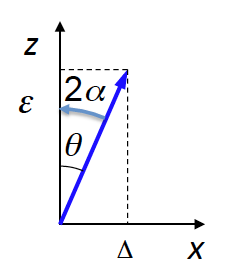
\includegraphics[height=4cm]{rot}
\end{figure}

\noindent

\noindent  Now  we perform  a  transformation  to  rotate the  state  by
$ 2\alpha = \theta $

  \begin{equation}
    \mathbf{U=e^{i\frac{\theta}{2}\sigma_y}} =  \cos(\alpha)\mathbb{I}+i\sin(\alpha)\sigma_y
  \end{equation}

  \noindent to rotate  the basis in this  plane.  \red{\textbf{Note that
      the transformation uses an angle HALF of the required turn}}.  The
  {time  independent Hamiltonian}  will be  transformed, and  evaluating
  using the commutation relations Eq.\eqref{uniComm1}

  \begin{equation}\label{uniRot}
    \begin{aligned}
      \mathcal{H}' & = U\mathcal{H}U^{\dagger} = U \bigg[-\frac{\Delta E}{2}\big(\sigma_z\cos(\theta)+\sigma_x\sin(\theta)\big)\bigg]\bigg[\cos(\theta/2)\mathbb{I}\red{-}i\sin(\theta/2)\sigma_y\bigg]\\
      & = U \bigg[\cos(\theta/2)\mathbb{I}+i\sin(\theta/2)\sigma_y\bigg]\bigg[-\frac{\Delta E}{2}\big(\sigma_z\cos(\theta)+\sigma_x\sin(\theta)\big)\bigg]\\
      & = UU\mathcal{H} =-\frac{\Delta E}{2} \bigg[\cos(\theta)\mathbb{I}+i\sin(\theta)\sigma_y\bigg]\bigg[\big(\sigma_z\cos(\theta)+\sigma_x\sin(\theta)\big)\bigg]\\
      & = -\frac{\Delta E}{2}\bigg[\cos^2(\theta)\sigma_z+\sin(\theta)\cos(\theta)\sigma_x+i\sin(\theta)\cos(\theta)\red{\sigma_y\sigma_z}+i\sin^2(\theta)\red{\sigma_y\sigma_x}\bigg]\\
      & = -\frac{\Delta E}{2}\bigg[\cos^2(\theta)\sigma_z+\sin(\theta)\cos(\theta)\sigma_x+i\sin(\theta)\cos(\theta)\red{i\sigma_x}+i\sin^2(\theta)\red{-i\sigma_z}\bigg]\\
      & = -\frac{\Delta E}{2}\sigma_z,
    \end{aligned}
  \end{equation}


  \noindent with  eigenstates $ \iket{\tilde{0}}, \iket{\tilde{1}}  $ at
  energies $  -\Delta E/2, +\Delta  E/2 $ respectively.   Recalling that
  the transformation we applied was

  \begin{equation}\label{uniTransform}
    \tilde{\Psi} = U\Psi \quad\Rightarrow\quad \Psi = U^{\dagger}\tilde{\Psi},
  \end{equation}

  \noindent in the initial eigenbasis, the two states will read

  \begin{equation}\label{uniInitial}
    \begin{aligned}
      \iket{0}_{\text{initial}}     &    =     U^{\dagger}\ket{\tilde{0}}    =
      \bigg(\cos(\theta/2)\mathbb{I}+i\sin(\theta/2)\sigma_y\bigg)\begin{pmatrix}
        1\\0
      \end{pmatrix} = \begin{pmatrix} \cos(\theta/2)\\\sin(\theta/2)
      \end{pmatrix} \\
      \iket{1}_{\text{initial}}      &       =      U^{\dagger}\ket{\tilde{1}}
      = \begin{pmatrix} -\sin(\theta/2)\\\cos(\theta/2)
      \end{pmatrix}.
    \end{aligned}
  \end{equation}


  \noindent  So ultimately,  rotating by  $ \theta/2  $ will  rotate the
  basis so as to cancel the interaction term.

 \subsection{Example application 2\label{subsec:Rabi}}
 Now  we have  a qubit  that  is driven  by a  resonant external  field,
 \red{this  time it  is not  a $  \Delta $  intractions as  the strength
   varies with time}

  \begin{equation}\label{app2}
    \mathcal{H} = -\frac{\hbar\omega_0}{2}\sigma_z-\hbar\Omega\cos(\omega_0 t)\sigma_x
  \end{equation}

  \noindent for which we shall try the unitary transformation

  \begin{equation}\label{app2Try}
    U(t) = \exp\left[-i\frac{\omega_0 t}{2}\sigma_z\right]
  \end{equation}

  \noindent resulting in the Hamiltonian

  \begin{equation}\label{app2New}
    \begin{aligned}
      \mathcal{H'} & = U\mathcal{H}U^{\dagger} - i\hbar U\dot{U}^{\dagger}\\
      & = -\frac{\hbar\omega}{2}e^{-i\omega_0t/2\sigma_z}\sigma_ze^{+i\omega_0t/2\sigma_z}-\hbar\Omega\frac{e^{i\omega t}+e^{-i\omega t}}{2}e^{-i\omega_0t/2\sigma_z}\sigma_xe^{i\omega_0t/2\sigma_z}- i\hbar e^{-i\omega_0t/2\sigma_z}\bigg(i\frac{\omega}{2}\sigma_z\bigg)e^{i\omega_0t/2\sigma_z}\\
      & = -\frac{\hbar\Omega}{2}\bigg(e^{i\omega t}+e^{-i\omega t}\bigg)e^{-i\omega_0t/2\sigma_z}\red{e^{(-1)i\omega_0t/2\sigma_z}\sigma_x}\\
      & = -\frac{\hbar\Omega}{2}\bigg(e^{i\omega t}+e^{-i\omega t}\bigg){e^{-i\omega_0t\sigma_z}\sigma_x}\\
      &      =-\frac{\hbar\Omega}{2}\bigg(e^{i\omega      t}+e^{-i\omega
        t}\bigg)\begin{pmatrix} e^{-i\omega_0t}&0\\0&e^{+i\omega_0t}
      \end{pmatrix}\begin{pmatrix}
        0&1\\1&0
      \end{pmatrix}\\
      &      =-\frac{\hbar\Omega}{2}\bigg(e^{i\omega      t}+e^{-i\omega
        t}\bigg)\begin{pmatrix} 0&e^{i\omega_0t}\\e^{-i\omega_0t}&0
      \end{pmatrix}
      \\
      &                           =-\frac{\hbar\Omega}{2}\begin{pmatrix}
        0&1+e^{2i\omega_0t}\\1+e^{-2i\omega_0t}&0
      \end{pmatrix}
      \\
      & \approx -\frac{\hbar\Omega}{2}\begin{pmatrix} 0&1\\1&0
      \end{pmatrix}
      \\
      & \approx -\frac{\hbar\Omega}{2}\sigma_x
    \end{aligned}
  \end{equation}

  \noindent where we have applied the RWA where we neglect fast rotating
  terms \begin{framed}\noindent which correspond to non conserved energy
    processes
  \end{framed}                     qubit                     Hamiltonian
  ($ \mathcal{H} =  -\frac{\hbar\omega}{2}\sigma_z $), implicitly taking
  into  account the  raw evolution  to concentrate  only on  the driving
  field contribution.

  \begin{center}
    Coupling of levels via radiation = RWA.
  \end{center}

  Now the evolution of the state

  \begin{equation}\label{app2Ev}
    U(t) = e^{-i\mathcal{H'}/\hbar t} = e^{i\Omega t/2\sigma_x}
  \end{equation}

  \noindent gives according to Eq.\eqref{uniPauli}

  \begin{equation}\label{app2State}
    \ket{\Psi} = U\ket{0} = \cos(\frac{\Omega t}{2})\ket{0}+e^{i\pi/2}\sin(\frac{\Omega t}{2})\ket{1}.
  \end{equation}

\begin{figure}[h]
  \centering 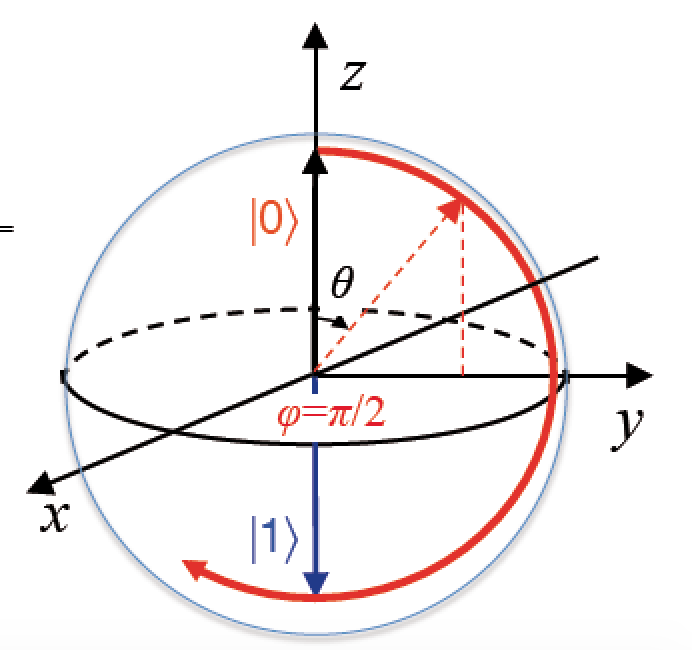
\includegraphics[height=2cm]{rotX}
\end{figure}

\noindent

\begin{framed}\noindent
  States  \iket{0}, \iket{1}  of the  same energy  (due to  the driving)
  interact with each other
\end{framed}
\noindent \textbf{It  may be  interesting to observe  the case  when the
  drive is changed}

  \begin{equation}\label{app2NewPhase}
    \hbar\Omega\cos(\omega t)\sigma_x \quad \rightarrow \quad \hbar\Omega\cos(\omega t+\mathbf{\phi})\sigma_x = \hbar\Omega\bigg[\cos(\omega t)\cos(\phi)-\sin(\omega t)\sin(\phi)\bigg]\sigma_x
  \end{equation}

  \noindent for which  the procedure for the cosine part  using the same
  unitary transformation Eq.\eqref{app2Try} gives

  \begin{equation}\label{app2Cos}
    -\frac{\hbar\Omega}{2}\cos(\phi)\sigma_x,
  \end{equation}

  \noindent                           while                          the
  $ \sin(\omega t) = i(e^{i\omega t}-e^{-i\omega t})/2 $ gets

  \begin{equation}\label{app2Sin}
    -\frac{\hbar\Omega}{2}\sin(\phi)\sigma_y,
  \end{equation}

  \noindent giving

  \begin{equation}\label{app2Combined}
    \mathcal{H'} = -\frac{\hbar\Omega}{2}\bigg(\sigma_x\cos\phi+\sigma_y\sin\phi\bigg)
  \end{equation}


 \subsection{Qubit operations}
 In the previous section, the qubit system was subjected to a field that
 induced rotation about  the x-axis.  In a similar way,  one can perform
 qubit operations about other axes

 {\footnotesize \begin{table}[h]
     \begin{center}
       \begin{tabular}{|c|c|c|c|c|}
         \hline \textbf{Axis} & \textbf{Field operator $ \mathcal{H} $} & \textbf{Unitary evolution}$ U=\exp\left[i\mathcal{H}t/\hbar\right] $ & $ \mathbf{t=\frac{\pi}{\Omega}} $& $ \mathbf{t=\frac{\pi}{2\Omega}} $\\
         X&$ -\frac{\hbar\Omega}{2}\sigma_x $ & $ \begin{pmatrix}
           \cos{\Omega t/2} & -i\sin{\Omega t/2}\\-i\sin{\Omega t/2}&\cos{\Omega t/2}
         \end{pmatrix} $ & NOT = $\begin{pmatrix} 0 & -i \\-i&0
         \end{pmatrix} $ &\\
         Y&$         -\frac{\hbar\Omega}{2}\sigma_y          $         &
                                                $        \begin{pmatrix}
                                                    \cos{\Omega  t/2}  &
                                                                       -\sin{\Omega
                                                                         t/2}\\\sin{\Omega
                                                           t/2}&\cos{\Omega
                                                                 t/2}
                                                             \end{pmatrix}
                                                                 $ &  FLIP =
                                                                     $\begin{pmatrix}
                                                                       0   &  -1
                                                                       \\1&0
                                                                     \end{pmatrix}
                                                                            $  &   H  =
                                                                                 $
                                                                                 \frac{1}{\sqrt{2}}\begin{pmatrix}
                                                                                   1   &  -1
                                                                                   \\1&1
                                                                                 \end{pmatrix} $\\
         Z&$         -\frac{\hbar\Omega}{2}\sigma_z          $         &
                                                $        \begin{pmatrix}
                                                    e^{-i\Omega  t/2}  &
                                                                       0\\0&e^{i\Omega
                                                                             t/2}
                                                                         \end{pmatrix}
                                                                             $&$\begin{pmatrix}
                                                                               -i&0\\0&i
                                                                             \end{pmatrix}$&\\\hline
       \end{tabular}
     \end{center}
   \end{table}}
 \newpage
